\documentclass{beamer}
\usepackage[utf8]{inputenc}
\usepackage[T1]{fontenc}
\usepackage[brazilian]{babel}
\usepackage{lmodern}
\usetheme{default}
\usecolortheme{beaver}
\usepackage{graphicx,xcolor}

\beamertemplatenavigationsymbolsempty

\title{Princípios Gerais e Erros}
\author
{
	Prof. Jonathan Esteban Arroyo Silva	
}
\institute
{
	Departamento de Ciência da Computação\\
	Universidade Federal de São João del-Rei\\
	\texttt{silva.jea@ufsj.edu.br}
}
\date{}
\logo{\includegraphics[width=0.2\linewidth]{../ufsj-logo-site}}

\begin{document}
	
\begin{frame}[plain]
    \maketitle
\end{frame}

\begin{frame}[plain]
	\frametitle{Sumário}
	\tableofcontents
\end{frame}

\section{Introdução}

\begin{frame}
	\frametitle{O que é Computação Científica?}
	\begin{itemize}
		\item Desenvolver e analisar \textcolor{red}{algoritmos} para resolver, de forma numérica, problemas \textcolor{green}{matemáticos} que surgem na \textcolor{blue}{ciência e engenharia}
		\begin{flushright}
			- \textit{Michael T. Heath}
		\end{flushright}
		\begin{figure}
			\centering
			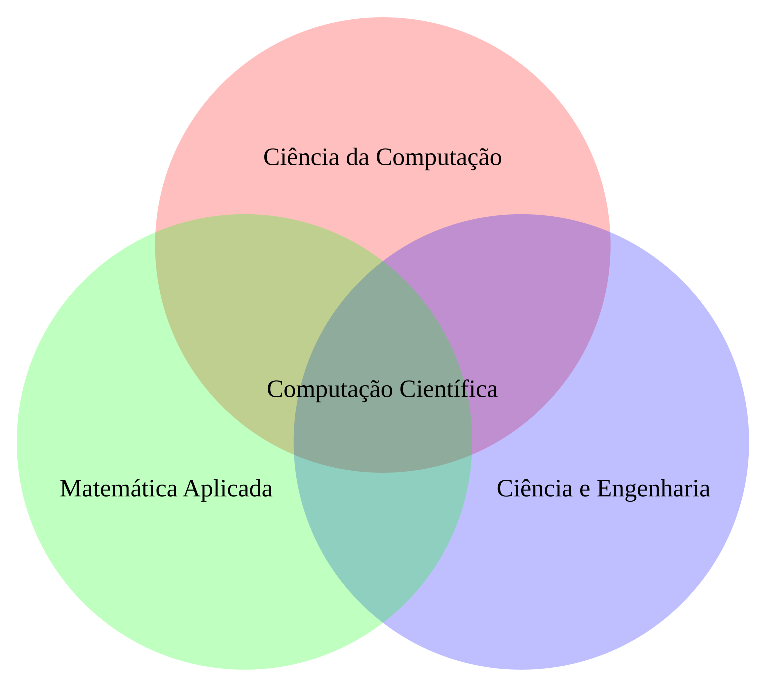
\includegraphics[width=0.6\linewidth]{Figuras/Computacao_cientifica}
			\label{fig:computacaocientifica}
		\end{figure}
	\end{itemize}			
\end{frame}

\begin{frame}
	\frametitle{Exemplos}
	\begin{figure}
		\centering
		\includegraphics[width=0.4\linewidth]{Figuras/numerical-simulation-01}
		\includegraphics[width=0.3\linewidth]{Figuras/numerical-simulation-02}\\
		\includegraphics[width=0.3\linewidth]{Figuras/numerical-simulation-03}
		\includegraphics[width=0.3\linewidth]{Figuras/numerical-simulation-04}
		\label{fig:exemplos}
	\end{figure}
\end{frame}

\begin{frame}
	\frametitle{O que é Computação Científica?}
	\begin{itemize}
		\item Para que serve computação científica?
		\begin{itemize}
			\item Simulação preditiva de fenômenos naturais
			\item Prototipagem virtual de projetos de engenharia
			\item Análise de dados
		\end{itemize}
		\item Diferentes aspectos da computação científica:
		\begin{itemize}
			\item Trabalhar com quantidades \textit{continuas} que são geralmente medidas com números reais (por exemplo: tempo, distância, velocidade, temperatura, densidade, pressão)
			\item Avaliar os efeitos das \textit{aproximações} utilizadas
		\end{itemize}
	\end{itemize}			
\end{frame}

\begin{frame}
	\frametitle{O que é Cálculo numérico?}
	Uma disciplina introdutória para \textit{Computação científica}
	\begin{itemize}
		\item Compreender como os números são representados nas calculadoras e computadores
		\item Apresentar os efeitos de utilizar \textit{aproximações}
		\item Conhecer os algoritmos clássicos para resolução de problemas numéricos
		\item Comparação e critério na escolha da \textit{melhor} opção possível
	\end{itemize}	
\end{frame}

\begin{frame}
	\frametitle{Solução Analítica $\times$ Solução Numérica}
	\begin{itemize}
		\item Solução Analítica:
		\begin{itemize}
			\item Representação numérica exata ou simbólica da solução
			\item Exemplo: Fórmula de Bháskara
		\end{itemize}
		\item Solução numérica:
		\begin{itemize}
			\item Representação computacional ou aproximada da solução
			\item Exemplo: Algoritmo de Eudoxo
		\end{itemize}
	\end{itemize}	
\end{frame}

\begin{frame}[plain]
	\centering\huge
	\bigskip
	\bigskip
	\bigskip
	\textbf{Por quê estudar soluções aproximadas?}
\end{frame}

\begin{frame}[plain]
	\centering\Large
	\emph{I’ve learned that, in the description of Nature, one has to tolerate \textbf{approximations}, and that work with approximations can be \textbf{interesting} and can sometimes be \textbf{beautiful}.\\
	\begin{flushright}
		- P. A. M. Dirac
	\end{flushright}
	\bigskip
	\bigskip	
	{\large Aprendi que, ao descrever a Natureza, é preciso tolerar \textbf{aproximações}, e que o trabalho com aproximações pode ser \textbf{interessante} e, por vezes, \textbf{belo}.}
	}
\end{frame}

\begin{frame}
	\frametitle{Descrevendo a Natureza}
	\begin{figure}
		\centering
		\includegraphics[width=0.7\linewidth]{Figuras/Solucao_problema}
		\label{fig:solucaoproblema}
	\end{figure}
\end{frame}

\begin{frame}
	\frametitle{Como resolver um problema numérico?}
	Para resolver um problema numérico, é necessário entender bem cada uma das três etapas:
	\begin{itemize}
		\item Método matemático: uma descrição matemática sobre o processo de solução
		\item Algoritmo: um passo-a-passo de como executar o método (Pseudocódigo)			
		\item Implementação: uma instanciação particular do algoritmo (utilizando alguma linguagem de programação)
	\end{itemize}
\end{frame}

\section{Sistema de ponto flutuante}

\begin{frame}
	\frametitle{Ponto flutuante}
	A representação de ponto flutuante é baseada na notação científica. Nessa notação um numero real não nulo $ x $ é expresso por:
	\begin{equation*}
		x = \pm d \times \beta^{e}
	\end{equation*}
	em que 
	\begin{itemize}
		\item $ d $ representa a mantissa;
		\item $ \beta $ representa a base do sistema de numeração
		\item $ e $ representa o expoente
	\end{itemize}	
\end{frame}

\begin{frame}
	\frametitle{Mantissa}
	A mantissa é a representação de um número da seguinte forma:
	\begin{equation*}
		(0. d_{1} d_{2} d_{3}\cdots d_{t})_{\beta}
	\end{equation*}
	e possuindo as seguintes propriedades:
	\begin{itemize}
		\item Os dígitos da mantissa $ 0 \leq d_{i} \leq \beta - 1 $, para $ i = 1, \ldots, t $ e com $ d_{1} \neq 0 $
		\item O número está \textbf{normalizado} quando $ d_{1} \neq 0 $
	\end{itemize}
\end{frame}

\begin{frame}
	\frametitle{Sistema de ponto flutuante}
	Um sistema de ponto flutuante é representado da forma:
	\begin{equation*}
		F(\beta, t, m, M)
	\end{equation*}
	em que:
	\begin{itemize}
		\item $ \beta $ é a base do sistema
		\item $ t $ é o número de dígitos da mantissa ou precisão
		\item $ m $ é o menor valor para o expoente $ e $
		\item $ M $	é o maior valor para o expoente $ e $
	\end{itemize}
\end{frame}

\begin{frame}
	\frametitle{Propriedades de um sistema de ponto flutuante}
	\begin{itemize}
		\item Um sistema de ponto flutuante é finito e \textit{discreto}
		\item Não todos os números reais são representados de forma exata
		\item A quantidade total de números de um sistema de ponto flutuante é dada por:
		\begin{equation*}
			2(\beta - 1)\beta^{t - 1}(M - m + 1) + 1
		\end{equation*}
		\item O menor número positivo normalizado é dado por: $ \mbox{UFL} = \beta^{m - 1} $
		\item O maior número representável é dado por: $ \mbox{OFL} = \beta^{M}(1 - \beta^{-t}) $
	\end{itemize}
\end{frame}

\begin{frame}
	\frametitle{Exemplo}
	\begin{itemize}
		\item Considerando o sistema de ponto flutuante $ F(10, 3, -3, 3) $, o número $ 12.5 $ será representado por:
		\begin{equation*}
			0.125 \times 10^{2}
		\end{equation*}
		\item O número de Euler, $ e = 2.718281\ldots $, será representado por:
		\begin{equation*}
			\begin{aligned}
				&0.271 \times 10^{1} \mbox{(com truncamento)}\\
				&0.272 \times 10^{1} \mbox{(com arredontamento)}
			\end{aligned}
		\end{equation*}
	\end{itemize}	
\end{frame}

\begin{frame}
	\frametitle{Exemplo}
	\begin{itemize}
		\item Considerando o sistema de ponto flutuante $ F(10, 3, -3, 3) $, todo número $ x $ tal que $\mbox{UFL} \leq | x | \leq \mbox{OFL}$ pode ser representado no sistema, sendo com arredondamento ou truncamento
		\item Se $ |x| < \mbox{UFL} $, o número não pode ser representado no sistema, ocorrendo o erro chamado de \textbf{underflow}, (e.g., $ 0.517 \times 10^{-8} $)
		\item Se $ |x| > \mbox{OFL} $, o número não pode ser representado no sistema, ocorrendo o erro chamado de \textbf{overflow}, (e.g., $ 0.725 \times 10^{9} $)
	\end{itemize}	
\end{frame}

\begin{frame}
	\frametitle{Operações aritméticas em ponto flutuante}
	As propriedades aritméticas não são verdadeiras para todos os casos em sistemas de ponto flutuante:
	\begin{equation*}
		\begin{aligned}
			&\mbox{Associatividade: } (a + b) + c = a + (b + c)\\
			&\mbox{Distributividade: } a (b + c) = ab + ac		
		\end{aligned}
	\end{equation*}
\end{frame}

\begin{frame}
	\frametitle{Exemplo}
	Considerando o sistema de ponto flutuante $ F(10, 3, m, M) $ com arredondamento, verifique se:
	\begin{itemize}
		\item $ (11.4 + 3.18) + 5.05 = 11.4 + (3.18 + 5.05) $
		\item $ 5.55(4.45 - 4.35) = 5.55\cdot 4.45 - 5.55\cdot4.35$
	\end{itemize}
\end{frame}

\section{Erros}

\begin{frame}
	\frametitle{Tipos de erros}
	Sendo $ \tilde{x} $ uma aproximação de $ x $, definimos como:
	\begin{itemize}
		\item Erro absoluto:
		\begin{equation*}
			\mbox{EA}(\tilde{x}) = |x - \tilde{x}|
		\end{equation*}
		\item Erro relativo:
		\begin{equation*}
			\mbox{ER}(\tilde{x}) = \frac{|x - \tilde{x}|}{|\tilde{x}|} = \frac{\mbox{EA}(\tilde{x})}{|\tilde{x}|}
		\end{equation*}
		desde que $ \tilde{x} \neq 0 $
	\end{itemize}
\end{frame}

\begin{frame}
	\frametitle{Efeitos numéricos}
	Outros tipos de erros são encontrados quando se realiza operações ariméticas nas seguintes condições:
	\begin{itemize}
	\item Soma entre dois números com ordens muito distintas
	\item Subtração entre dois números de magnitudes semelhantes
	\end{itemize}
\end{frame}

\begin{frame}
	\frametitle{Exemplo}	
	Considerando o sistema de ponto flutuante $ F(10, 4, m, M) $ com arredondamento, realize as seguintes operações e compare os resultados com sua solução exata:
	\begin{itemize}
		\item $ 0.1 + 5000.0 $
		\item $ \sqrt{37} - \sqrt{36} $
	\end{itemize}
\end{frame}

\begin{frame}
	\frametitle{Conclusão}	
	Foram abordados os seguintes assuntos:
	\begin{itemize}
		\item Cálculo numérico como uma disciplina introdutória para \textit{Computação científica}
		\item Solução analítica $ \times $ Solução numérica
		\item Aritmética de ponto flutuante
		\item Tipos de erros em consequência de trabalhar com um sistema \textit{discreto} e finito
	\end{itemize}
\end{frame}

\begin{frame}[plain]
\bigskip
\bigskip
\bigskip
\bigskip
\bigskip
\begin{figure}
	\centering
	
\includegraphics[width=0.9\linewidth]{../Luffy_v}
	\label{fig:luffyv}
\end{figure}
\end{frame}

\end{document}
